% fig_architecture_resblock.tex
% Figure 3.3 -- ResBlock detail
\begin{figure}[htbp]
\centering
\resizebox{0.88\linewidth}{!}{%
\begin{tikzpicture}[
  >=Stealth,
  every node/.style={font=\small},
  imgblk/.style={inner sep=0pt, outer sep=0pt},
  fmblk/.style={inner sep=0pt, outer sep=0pt},
  % Box heights reduced from 0.88 cm to 0.60 cm.
  % Node spacing 1.1 cm → visible arrow gap = 0.50 cm.
  opbox/.style={draw=blue!60!black, fill=blue!10, rounded corners=3pt,
                minimum width=3.2cm, minimum height=0.60cm,
                align=center, line width=0.8pt},
  normbox/.style={draw=teal!65!black, fill=teal!9, rounded corners=3pt,
                  minimum width=3.2cm, minimum height=0.60cm,
                  align=center, line width=0.8pt},
  actbox/.style={draw=orange!65!black, fill=orange!9, rounded corners=3pt,
                 minimum width=3.2cm, minimum height=0.60cm,
                 align=center, line width=0.8pt},
  addnode/.style={draw=gray!65, fill=gray!13, circle,
                  minimum size=0.55cm, align=center, line width=0.8pt,
                  font=\normalsize},
  dimtag/.style={font=\fontsize{7}{8}\selectfont, text=black!60, align=center},
  arrmain/.style={->, line width=1.5pt, black!70},
  arrskip/.style={->, line width=1.2pt, blue!70, dashed},
]

% ── LEFT COLUMN: ResBlock vertical flow ─────────────────────────────

\node[dimtag] at (0,12.0) {$\mathbf{f}_{\mathrm{in}}$\;($H{\times}W{\times}C$)};
\node[imgblk] (fin_img) at (0,10.8)
  {\includegraphics[width=1.8cm,height=1.8cm,keepaspectratio]%
    {figures/arch/arch_input_noisy.png}};

\node[opbox]   (conv1) at (0,8.6)  {\textbf{Conv}\;$3{\times}3$,\;pad\;1};
\node[normbox] (gn1)   at (0,7.5)  {\textbf{GroupNorm}\;($G{=}8$)};
\node[actbox]  (gelu1) at (0,6.4)  {\textbf{GELU}};
\node[opbox]   (conv2) at (0,5.3)  {\textbf{Conv}\;$3{\times}3$,\;pad\;1};
\node[normbox] (gn2)   at (0,4.2)  {\textbf{GroupNorm}\;($G{=}8$)};
\node[addnode] (add)   at (0,3.0)  {$+$};
\node[actbox]  (gelu2) at (0,2.0)  {\textbf{GELU}};

\node[dimtag, anchor=west] at (1.7,1.1) {$\mathbf{f}_{\mathrm{res}}$\;($H{\times}W{\times}C$)};
\node[imgblk] (fout_img) at (0,-0.1)
  {\includegraphics[width=1.8cm,height=1.8cm,keepaspectratio]%
    {figures/arch/arch_input_noisy.png}};
\node[dimtag, below=3pt of fout_img]
  {same spatial resolution\;and\;channel\;count};

% ── Flow arrows ──────────────────────────────────────────────────────
\draw[arrmain] (fin_img.south) -- (conv1.north);
\draw[arrmain] (conv1.south)   -- (gn1.north);
\draw[arrmain] (gn1.south)     -- (gelu1.north);
\draw[arrmain] (gelu1.south)   -- (conv2.north);
\draw[arrmain] (conv2.south)   -- (gn2.north);
\draw[arrmain] (gn2.south)     -- (add.north);
\draw[arrmain] (add.south)     -- (gelu2.north);
\draw[arrmain] (gelu2.south)   -- (fout_img.north);

% ── Residual skip: fin_img.west → down → add.west ────────────────────
\draw[arrskip]
  (fin_img.west)
  -- ++(-1.1, 0)
  -- node[left, font=\fontsize{7}{8}\selectfont, xshift=-2pt]
       {residual $\mathbf{f}_{\mathrm{in}}$}
     ++(0, -7.8)
  -| (add.west);

% ── RIGHT PANEL: real feature map with 3×3 window annotation ─────────
\begin{scope}[shift={(3.5, 5.0)}]
  \node[fmblk] at (1.35,1.35)
    {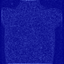
\includegraphics[width=2.7cm,height=2.7cm]{figures/arch/featmap_256.png}};
  \draw[white, line width=0.3pt, opacity=0.7, step=0.45] (0,0) grid (2.7,2.7);
  \fill[blue!50, opacity=0.28] (0.45,0.45) rectangle (1.80,1.80);
  \draw[white, line width=2.2pt] (0.45,0.45) rectangle (1.80,1.80);
  \draw[cyan!90!white, line width=1.5pt] (0.45,0.45) rectangle (1.80,1.80);
  \begin{scope}[shift={(1.95,0.0)}]
    \fill[blue!35] (0,0) rectangle (0.75,0.75);
    \draw[white, line width=0.5pt, step=0.25] (0,0) grid (0.75,0.75);
    \fill[cyan!80, opacity=0.9] (0.25,0.25) rectangle (0.50,0.50);
    \node[font=\fontsize{5}{5}\selectfont, white, below=1pt] at (0.375,-0.01)
      {kernel};
  \end{scope}
  \node[font=\fontsize{7}{8}\selectfont, white, above=3pt] at (1.35,2.7)
    {Feature map $H{\times}W{\times}C$};
  \node[font=\fontsize{7}{8}\selectfont, white, below=2pt] at (1.35,0.0)
    {$3{\times}3$ sliding window (highlighted)};
  % Arrow ends at scope x=0 = image left boundary; tip not inside image
  \draw[->, gray!70, line width=0.8pt] (-0.3,0.7) -- (0.0,1.1);
  \node[font=\fontsize{7}{8}\selectfont, text=black!75, anchor=east] at (-0.3,0.7)
    {receptive field};
\end{scope}

\draw[gray!50, dashed, line width=0.6pt] (conv1.east) -- (3.5, 6.7);

\end{tikzpicture}%
}
\caption[ResBlock convolutional component architecture]{%
  \textbf{ResBlock -- convolutional component of the HybridBlock.}
  The input feature map $\mathbf{f}_{\mathrm{in}}$ ($H{\times}W{\times}C$, illustrated
  by a lung radiograph thumbnail) passes through two sequential $3{\times}3$
  convolutions each followed by GroupNorm ($G{=}8$ groups) and GELU activation.
  A residual shortcut (blue dashed arrow) adds the unchanged input to the second
  GroupNorm output before a final GELU, producing $\mathbf{f}_{\mathrm{res}}$ at the
  same spatial resolution and channel count as the input.
  \textit{Right:} real convolutional feature map (sampled from the network's first
  encoder stage) with the $3{\times}3$ sliding window highlighted in cyan; every
  output location integrates a local $3{\times}3$ neighbourhood, enabling
  precise local texture and edge extraction.}
\label{fig:arch:resblock}
\end{figure}
